\section{Dealing with imbalanced data}

\subsection{Motivation}

\begin{frame}\frametitle{\subsecname}

\only<1>{
Proportion of class labels in the dataset is not uniform.
Not the same as ``easy vs. difficult'' classes. This is only about class frequency.
}

\slidesonly{\vspace{-5mm}}

\begin{figure}[ht]
     \centering
     \savebox{\imagebox}{
	 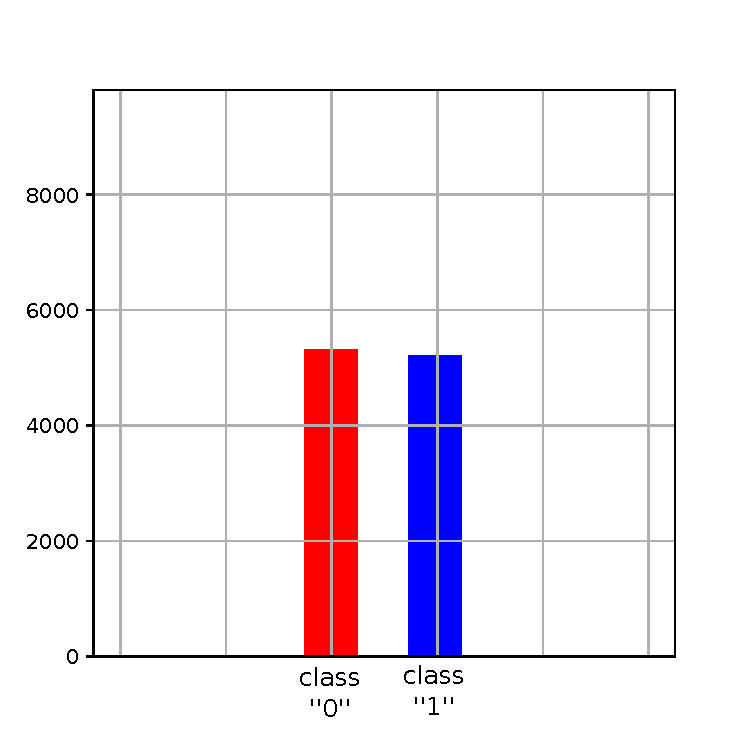
\includegraphics[width=0.37\textwidth]{img/hist_balanced}}%
     \begin{subfigure}[t]{0.37\textwidth}
         \centering
         \usebox{\imagebox}% Place largest image
         \caption{balanced $\approx 1:1$}
     \end{subfigure}
     \hspace{2mm}
     \begin{subfigure}[t]{0.37\textwidth}
         \centering
         \raisebox{\dimexpr.5\ht\imagebox-.5\height}{% Raise smaller image into place
         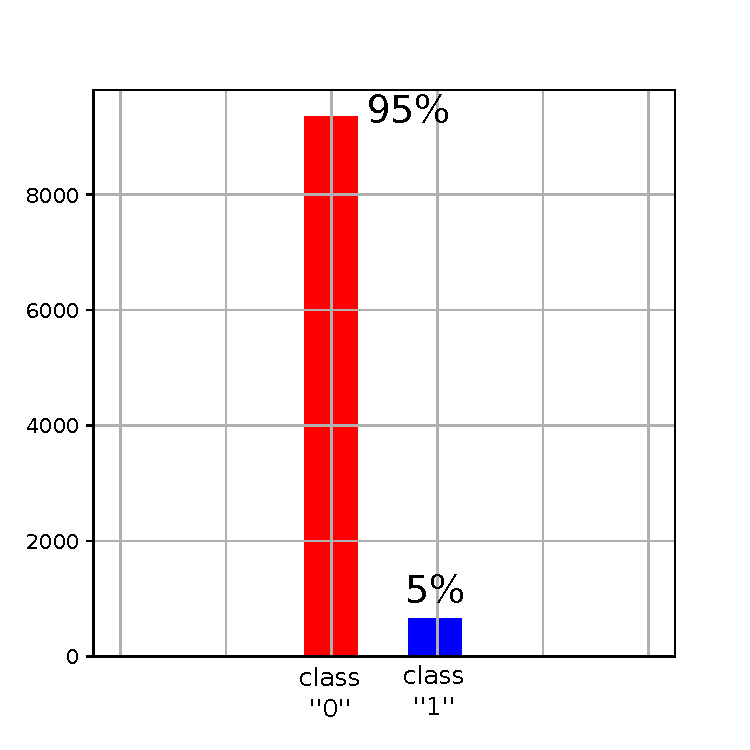
\includegraphics[width=0.99\textwidth]{img/hist_imbalanced}
         }
         \caption{highly unbalanced}
         \label{fig:linear}
     \end{subfigure}
\end{figure} 

\only<2>{     
A strong imbalance leads to the classifier learning a trivial solution that minimizes the average cost over the training samples.
}
\only<2,3>{
\begin{equation}
E^T = \sum_{\alpha=1}^p e^{(\alpha)}
\end{equation}
}
\only<3>{
By always predicting ``0'' it will be correct 95\% of the time.
}
\end{frame}

\subsection{Confusion matrix}

\begin{frame}\frametitle{\subsecname}

The confusion matrix differentiates between the types of mistakes a classifier makes.

\begin{tabular}{ll|l|l|l}
\cline{3-4}
												  &          & \multicolumn{2}{c|}{Ground truth label}                        &  \\ \cline{3-4}
												  &          & \multicolumn{1}{c|}{Positive} & \multicolumn{1}{c|}{Negative}  &  \\ \cline{3-4}
												  &          & \multicolumn{1}{c|}{``Cat''} & \multicolumn{1}{c|}{``not Cat''}  &  \\ \cline{1-4}
\multicolumn{1}{|r|}{\multirow{2}{*}{Prediction}} & Positive & \textbf{T}rue \textbf{P}ositives & \textbf{F}alse \textbf{P}ositives &  \\ \cline{2-4}
\multicolumn{1}{|r|}{}                            & Negative &  \textbf{F}alse \textbf{N}egatives & \textbf{T}rue \textbf{N}egatives &  \\ \cline{1-4}
												  &          & \multicolumn{1}{c|}{P} & \multicolumn{1}{c|}{N}  &  \\ \cline{3-4}
\end{tabular}	


\end{frame}

\subsection{Performance metrics}

\begin{frame}\frametitle{\subsecname}

\mode<presentation>{
\begin{tabular}{ll|l|l|l}
\cline{3-4}
												  &          & \multicolumn{2}{c|}{Ground truth label}                        &  \\ \cline{3-4}
												  &          & \multicolumn{1}{c|}{Positive} & \multicolumn{1}{c|}{Negative}  &  \\ \cline{3-4}
												  &          & \multicolumn{1}{c|}{``Cat''} & \multicolumn{1}{c|}{``not Cat''}  &  \\ \cline{1-4}
\multicolumn{1}{|r|}{\multirow{2}{*}{Prediction}} & Positive & \textbf{T}rue \textbf{P}ositives & \textbf{F}alse \textbf{P}ositives &  \\ \cline{2-4}
\multicolumn{1}{|r|}{}                            & Negative &  \textbf{F}alse \textbf{N}egatives & \textbf{T}rue \textbf{N}egatives &  \\ \cline{1-4}
												  &          & \multicolumn{1}{c|}{P} & \multicolumn{1}{c|}{N}  &  \\ \cline{3-4}
\end{tabular}	

}

\begin{equation}
\text{Accuracy } \corresponds
 \text{ \# of correct classifications } 
 = \frac{TP+TN}{P+N}
\end{equation}

\only<2>{
\slidesonly{
{\placeimage{12}{1}{img/hist_imbalanced}{width=3cm}}
}

In our imbalanced example:
\begin{equation}
\frac{TP+TN}{P+N} = \frac{0+9500}{500+9500} = 0.95
\end{equation}

Accuracy is a misleading metric when the classes are imbalance.
}

\only<3>{
Other metrics:

How many of the positive labels did we get:

\begin{equation}
\text{sensitivity (recall) }
 = \frac{TP}{P}
\end{equation}

and how often were we correct, whenever we predicted positive?

\begin{equation}
\text{precision }
 = \frac{TP}{TP+FP}
\end{equation}

Combine recall and precision into:

\begin{equation}
\text{F1 score }
 = 2 \frac{\mathrm{recall} \times \mathrm{precision}}{\mathrm{recall} + \mathrm{precision}}
\end{equation}

Similarly, for the negative class. How many of the negative class did we get:

\begin{equation}
\text{specificity}
 = \frac{TN}{N}
\end{equation}


Combine recall and specificity into:


\begin{equation}
\text{Balanced Accuracy }
 = \frac{1}{2} (\mathrm{recall} + \mathrm{specificity})
\end{equation}

}

\end{frame}

\subsection{Further considerations}

\begin{frame}\frametitle{\subsecname}

\begin{enumerate}
\item
Is there only one recall value for my classifier that predicts with\\
 $y(\vec x) \in \lbrack0,1\rbrack$ (or $\lbrack-1,1\rbrack$, $(0,1)$)?
\item
What if the proportions in my training set is different from that of the validation/test set?
\end{enumerate}


\end{frame}

\subsubsection{Calibration}

\begin{frame}\frametitle{\subsubsecname}

Calibration: finding an operating point by adjusting the threshold that takes converts the prediction of classifier into a hard decision.

General procedure:
\begin{enumerate}
\item train binary classifier (assuming $y(\vec x) \in \lbrack0,1\rbrack$)
\item make predicitons on the test set (selecting an operating point counts as a hyperparameter selection)
\item Save ``probabilistic'' output, no thresholding.
\item for threshold $\mathrm{thr} \in \lbrack0,1\rbrack$ do:
\begin{enumerate}
	\item assign predictions to classes using current threshold $\mathrm{thr}$
	\item compute confusion matrix (e.g. $TP$ and $FP$)
	\item[]repeat
\end{enumerate}
\item Compute metrics as a function of $\mathrm{thr}_i$
\end{enumerate}



\end{frame}

\begin{frame}
Example for the calibration procedure: \emph{Receiver operating characteristics (ROC)}. Keep track of $TP$ and $FP$ as a function of different threshold values.

\begin{figure}[h]
	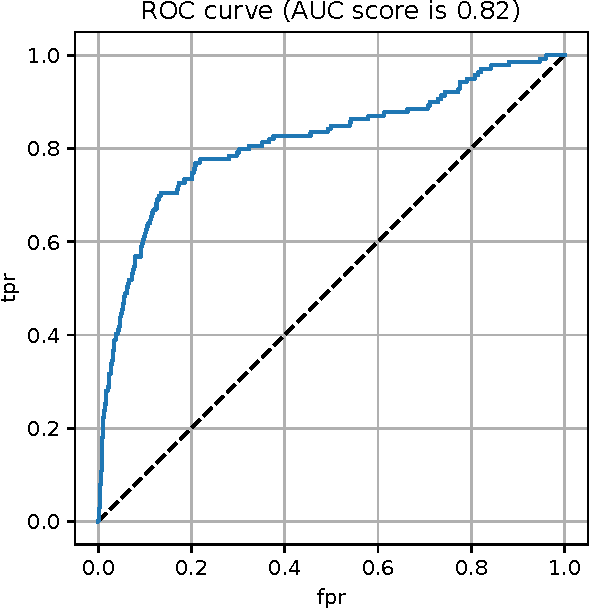
\includegraphics[width=0.35\textwidth]{img/curves_roc}
	\caption{ROC curve}
\end{figure}

\only<1>{
The higher the area under curve (ROC AUC) the better the classifier.

\question{What does the dashed diagonal line represent?}

}
\only<2>{

\textbf{But}\\
At the end of the day I need to pick an operating point.

\question{What criterion could I use to favor one threshold over and other?}
}

\end{frame}

\begin{frame}

What if the proportions in my training set is different from that of the validation/test set? Which metrics are robust to changes in proportions between different splits of the data.\footnote{cf. jupyter notebook on ISIS for a comparison of different metrics under different conditions.}

\slidesonly{\vspace{-2mm}}

\begin{figure}[h]
	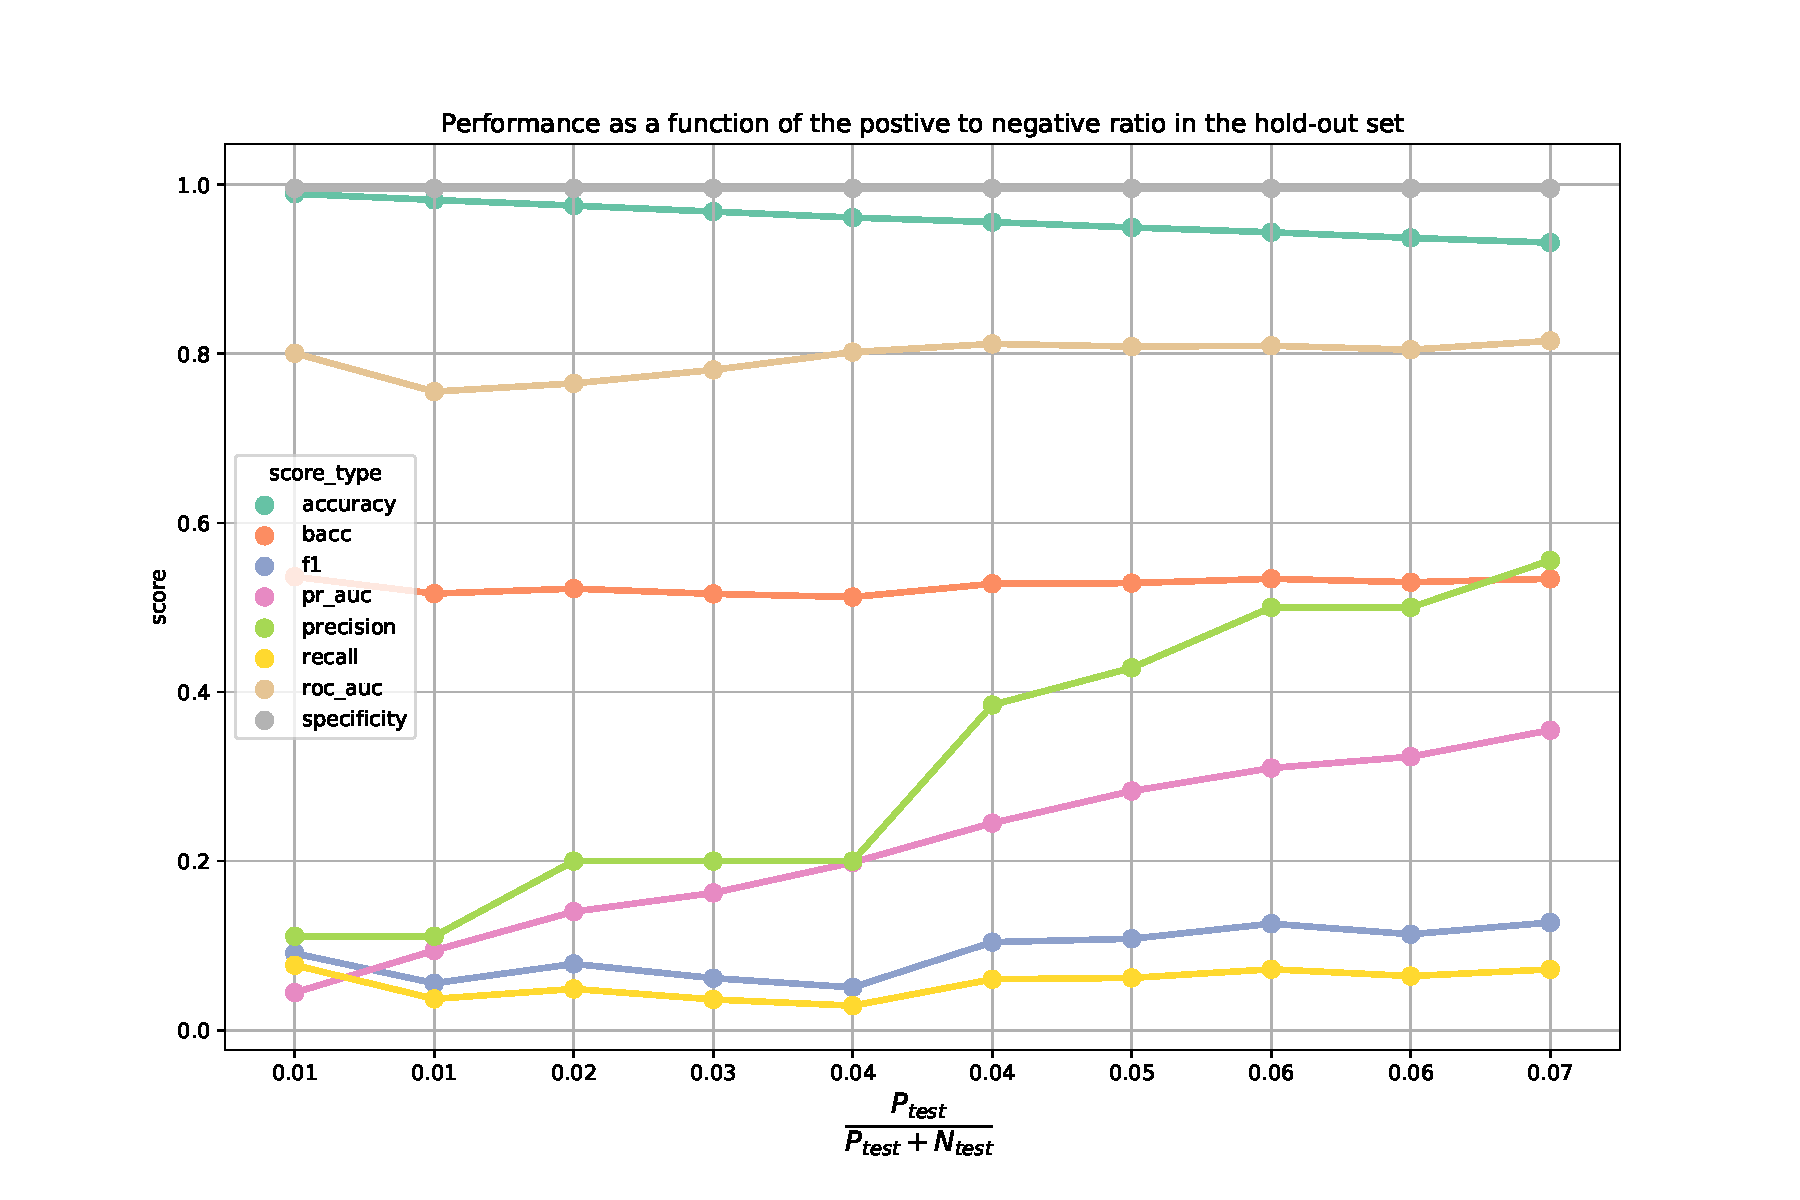
\includegraphics[width=0.8\textwidth]{img/compare_metrics}
	\mode<article>{
	\caption{Comparing metrics under different conditions}
	}
\end{figure}



\end{frame}

\begin{frame}

All we did so far is measure generlization performance and tune our operating point.

\question{Is there anything else we can do about imabalanced data?}

\pause

\begin{enumerate}
\item Train the classifier on a synthetically balanced dataset by
\begin{itemize}
\item subsampling from the majority class (no one likes to throw away data)
\item oversampling the minority class
\end{itemize}

\question{Any downsides to oversampling?}

\pause

- the resulting dataset could be too large.
\item class weighted loss function:
e.g. weighted cross entropy:
\begin{equation}
e^{(\alpha)} = -\gamma y_T^(\alpha) \ln(y^{(\alpha)}) - \beta (1-y_T^{(\alpha)}) \ln(1-y^{(\alpha)})
\end{equation}
where $\beta$ and $\gamma$ represent ``class weights''
\end{enumerate}


\end{frame}



